\documentclass[12pt,letterpaper]{article}
\usepackage[utf8]{inputenc}
\usepackage[spanish,mexico]{babel}
\usepackage{amsmath}
\usepackage{amsfonts}
\usepackage{amssymb}
\usepackage{amsmath}
\usepackage[lmargin=3cm,rmargin=3cm,tmargin=3cm,bmargin=3cm]{geometry}

\usepackage{hyperref}
\usepackage{graphicx}
\usepackage{float}
\begin{document}

\title{Actividad 1: Preparando documentos científicos con LATEX}
\author{Luisa Fernanda Orci Fernandez.}
\date{22 de Enero del 2016}

\maketitle

\section*{Péndulo}
Las ecuaciones de un péndul son en general muy complicadas. Simplificando las condiciones iniciales, estas ecuaciones también se puden simplificar, este es el caso de un péndulo simple.

\section{Péndulo gravitatorio simple}
El péndulo simple es una idealización de un péndulo real pero dentro de un sistema aislado haciendo uso de las siguientes suposiciones:

\begin{itemize}

\item El cable o la cuerda del péndulo se considera sin masa, no extendible y siempre tenso/a.
\item Se considera como masa puntual.
\item El movimiento solo ocurre en dos dimensiones (es bidimensional).
\item Se desprecia la fricción o la resistencia del aire.
\item El campo gravitacional es uniforme.
\item El soporte no se mueve.


\end{itemize}

La ecuación diferencial que representa el movimiento de un péndulo simple es la siguiente:

\begin{equation}
\frac{d^2}{dt^2} + \frac{g}{l}\sin\theta = 0
\end{equation}

Donde $g$ represneta la gravedad, $l$ es la longitud del péndulo y $\theta$ es el ángulo de desplazamiento.

\subsection{Derivación de "Fuerza" de la ecuación 1}
Considerando la figura 1, nos muestra las fuerzas que actuan sobre un péndulo simple. El ángulo $\theta$ se toma en radianes, esto es crucial para la fórmula. La flecha azul nos indica la fuerza gravitacional que actua sobre la bolita del péndulo. 
Considerando la segunda ley de Newton: $$ F = ma $$ donde $F$ es la suma de las fuerzas que actuan sobre el objeto, $m$ es la masa y $a$ la aceleración.

\begin{eqnarray}
\nonumber F = -mg\sin\theta = ma \\
\nonumber a = -g\sin\theta 
\end{eqnarray}

donde g es la aceleración de la gravedad cerca de la superficie de la tierra. El signo negativo indica que $\theta y a$ siempre apuntan en direcciones opuestas.

\begin{figure}
\begin{center}
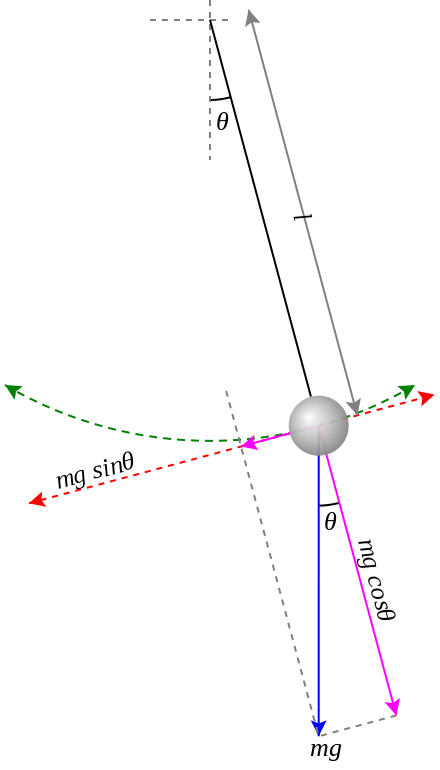
\includegraphics[scale=.3]{Pendulum.png}
\caption{Figura 1: Diagrama de fuerza de un Péndulo Simple}
\end{center}

\end{figure}

La aceleración líneal $a$ a tráves del eje de las $x's$ se puede relacionar al cambio del ángulo $\theta$ con la fórmula de la longitud de arco; $s$ esta es:

\begin{eqnarray}
\nonumber s = l\theta \\
\nonumber v = \frac{ds}{dt} = l\frac{d\theta}{dt} \\
\nonumber a = \frac{d^2 s}{dt^2} = l\frac{d^2 \theta}{dt^2}
\end{eqnarray}

Entonces: 

\begin{eqnarray}
\nonumber l\frac{d^2 \theta}{dt^2} = -g\sin\theta \\
\nonumber \frac{d^2 \theta}{dt^2} + \frac{g}{l}\sin\theta = 0
\end{eqnarray}

\subsection{Derivación de "Energía" de la ecuación 1}
La ecuación anterior también se puede obtener a través del principio de la conservación de la energía mécanica: cualquier objeto callendo de manera vertical a una distancia $ h $ adquirirá una energía cinética igual a la que se perdió con la caída. 
El cambio en la energía potencial está dado por: 
$$ \Delta U = mgh $$ 
El cambio en la enería cinética está dado por: 
$$ \Delta K = \frac{1}{2}mv^2 $$ 

Dado que no hay perdida de energía: 
$$ \frac{1}{2}mv^2 = mgh $$

Expresando a la velocidad de la siguiente forma: $$ v = \sqrt{2gh} $$  y la fórmula de la longitud del arco, esta ecuación puede reescribirse en terminos de $ \frac{d\theta}{dt} $.

\begin{figure}
\begin{center}
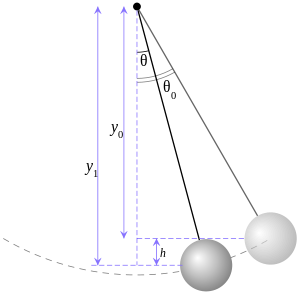
\includegraphics[scale=.3]{Pendulum2.png}
\caption{Figura 2: Trigonometría de un péndulo gravitatorio simple}
\end{center}
\end{figure}

Guíandonos con la figura 2, podemos llegar a la siguiente ecuación:

\begin{equation}
\frac{d\theta}{dt} = \sqrt{\frac{2g}{l}(cos\theta - cos\theta_0}
\end{equation}

Esta ecuación es también conocida como la primera intregral del movimiento y se puede diferenciar por la regla de la cadena y llegaríamos a la ecuación (1). 



\section{Aproximación con ángulos pequeños}

La ecuación diferencial dada anteriormente no se puede resolver de manera fácil, y no hay solución alguna que nos permita escribirla en terminos de funciones elementales. Pero añadiendo una restricción al tamaño de la amplitud de la oscilación, nos da una ecuación cuya solución se puede obtener de manera fácil, esta es, asumir que el ángulo es mucho mas pequeño que 1 radián:

 $$0 \ll 1$$
Esto lo sustituimos por $\sin\theta$ en la ecuación (1): $$ \sin\theta \approx \theta $$
Esto nos lleva a obtener la ecuación para un oscilador ármonico:

$$ \frac{d^2\theta}{dt^2} + \frac{g}{l}\theta = 0 $$
El error debido a la aproximación es de orden $\theta^3$.

Tomando en cuenta las condiciones iniciales $ \theta(0) = \theta_0 $, $\frac{d\theta}{dt}(0) = 0 $, la solución es: 

\begin{equation}
\nonumber \theta(t)= \theta_0 (\sqrt{\frac{g}{l}t})  \qquad \theta_0 \ll 1
\end{equation}

Este movimiento no es nada mas que el movimiento simple ármonico, donde $\theta_0$ es la semi amplitud de la oscilación. El periodo del movimiento, el tiempo para una oscilación completa es:

$$ T_0 = 2\pi \sqrt{\frac{l}{g}} \qquad \theta_0 \ll 1  $$
Esta ecuación también se conoce como la ley para el periodo de Christiaan Huygens's.

\subsubsection{Regla de oro para la longitud del péndulo}

La ecuación: 

$$ T_0 = 2\pi \sqrt{\frac{l}{g}} $$

también puede escribirse como: 

$$ l = \frac{g}{\pi^2} x \frac{T^2_0}{4} $$

Si se utilizan las unidades del sistema internacional, y si se asume que la medición fue tomada en la superficie de la tierra, entonces $ g \approx 9.8m/s^2$ y $ g/\pi^2 \approx 1 $, por lo tanto, las aproximaciones relativamente razonables para el periodo y la longitud serían:

\begin{eqnarray}
\nonumber l \approx \frac{T^2_0}{4}, \\
\nonumber T_0 \approx 2\sqrt{l}
\end{eqnarray}

Donde $T_0$ es el número de segundos entre dos "latidos", y $ l $ está medida en metros.


\section{Período de amplitud arbitraria}

Para aplitudes mas grandes que el pequeño ángulo de aproximación, se puede calcular el periodo exacto invirtiendo la ecuación para la velocidad angular obtenida del método de la energía, (ecuación 2);

$$ \frac{dt}{d\theta} = \sqrt{\frac{l}{2g}} \frac{1}{\sqrt{cos\theta - cos\theta_0}} $$

y despues podemos integrar para un ciclo completo, o para dos veces la mitad de ese ciclo, o para 4 veces el cuarto de ese ciclo, lo que nos lleva a: 

$$ T = 4\sqrt{\frac{l}{2g}} \int_{0}^{\theta_0}\frac{1}{\cos \theta - \cos \theta_0}d\theta $$.

Esta integral puede reescribirse en terminos de integrales elípticas: 

$$ T = 4\sqrt{\frac{l}{g}} F (\frac{\theta_0}{2}, \csc\frac{\theta_0}{2})\csc\frac{\theta_0}{2} $$ 

Donde $ F $ es la integral elíptica incompleta de la primera especie, la sustituimos y llegamos a la siguiente ecuación:

\begin{equation}
T = 4\sqrt{\frac{l}{g}} K (\sin^2(\frac{\theta_0}{2}))
\end{equation}

Donde K es la integral elíptica completa de la primera especie.


\subsection{Solución polinomial para la integral elíptica de Legendre}

\begin{figure}
\begin{center}
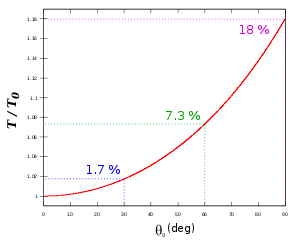
\includegraphics[scale=.3]{Pendulum3.png}
\caption{Figura 3: Derivación del "verdadero" periodo de un péndulo con ángulo pequeño de aproximación. Este valor se obtuvo usando Matlab}
\end{center}
\end{figure}

\begin{figure}
\begin{center}
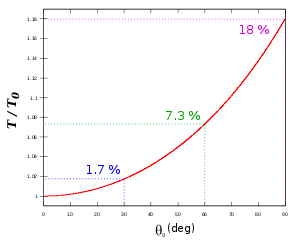
\includegraphics[scale=.3]{Pendulum3.png}
\caption{Figura 4: Errores relativos utilizando series de potencia}
\end{center}
\end{figure}
Dada la ecuación (3) y la solución del polinomio de Legendre  para la integral elíptica: 

$$ K(k) = \frac{\pi}{2} \{1 + (\frac{1}{2})^2 k^2 + (\frac{1\cdotp3}{2\cdotp4})^2 k^4 + \cdots + [\frac{(2n-1)!!}{(2n)!!}^2 k^{2n} + \cdots \} $$

donde $ n!! $ es el doble factorial.

La figura 4 nos muestra el error relativo utilizando la serie de potencias. 

\subsection{Solución para la integral elíptica utilizando sere de potencias}

Otra formulación para obtener el resultado anterior puede encontrarce en la serie de Maclaurin: 

$$ \sin\frac{\theta_0}{2} = \frac{1}{2}\theta_0 - \frac{1}{48}\theta^3_0 + \frac{1}{3840}\theta^5_0 - \frac{1}{645120}\theta^7_0 + \cdots . $$

\subsection{Solución media aritmética-geómetrica para la integral elíptica}

Dada la ecuación 3, y la solución media aritmética-geómetrica de la integral elíptica: 

$$ K(k) = \frac{\pi/2}{M(1-k, 1+k)} $$

donde $ M(x,y) $ es la media aritmética-geómetrica de $ x $ y $ y $. 

Esto nos lleva a una forumula aleternativa y que convergue mas rápido para el período:

$$ T = \frac{2\pi}{M(1, \cos(\theta_0/2))} \sqrt{\frac{l}{g}} $$ 

\begin{thebibliography}{widestlabel}
\bibitem{w} Wikipedia, https://en.wikipedia.org/wiki/Pendulum
\end{thebibliography}



\end{document}